\documentclass{standalone}
\usepackage[T1]{fontenc}
\usepackage[latin2]{inputenc}
\usepackage[english]{babel}
\usepackage{tikz}
\usepackage{times}
\usetikzlibrary{calc,through,backgrounds,positioning,fit}
\usetikzlibrary{shapes,arrows,shadows}
 

\begin{document}

 \begin{centering}

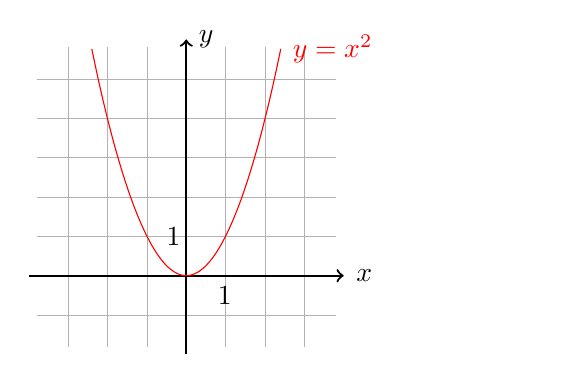
\begin{tikzpicture}[scale=1,inner sep=0.4mm]
\draw[step=5mm,draw=black!30!white,very thin] (-1.9,-0.9) grid (1.9,2.9);
\draw[thick] [->] (-2,0) -- (2,0) node [right=3pt] {$x$};
\node[text width = 4cm] at (1.75,0.5) {$1$};
\node[text width = 4cm] at (2.4,-0.25) {$1$};
\draw[thick][->](0,-1)--(0,3) node [right=3pt]{$y$};
\draw [red] (0,0) parabola (1.2, 2.88)node [right=3pt]  (0.5,0.5) {$y=x^2$};
\draw[red](0,0)parabola(-1.2,2.88);
\end{tikzpicture}
\end{centering}
\end{document}